\secframe{StuRa E-Mailverteiler} {
	Web-Adresse f\"ur die \"Ubersicht der E-Mailverteiler vom StuRa \url{https://lists.stura.htw-dresden.de}.
   \begin{figure}
	   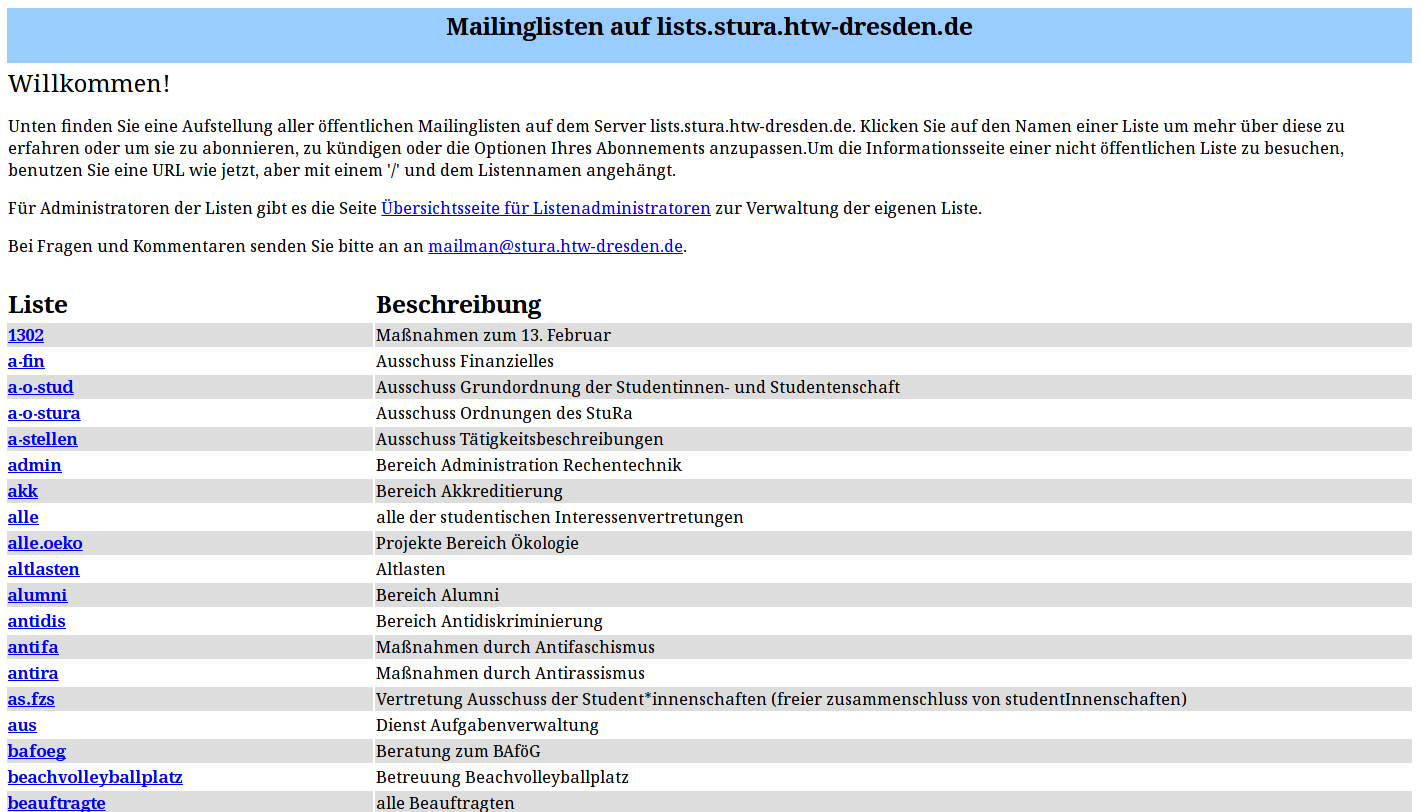
\includegraphics[width=\textwidth]{../images/lists_seite.png}
   \end{figure}

}
%% URL
%% Abbonieren/abbestellen
\subsecframe{Abbonieren} {
	\url{https://lists.stura.htw-dresden.de/listinfo/}\textbf{$<$Name der Liste$>$}
   \begin{figure}
	   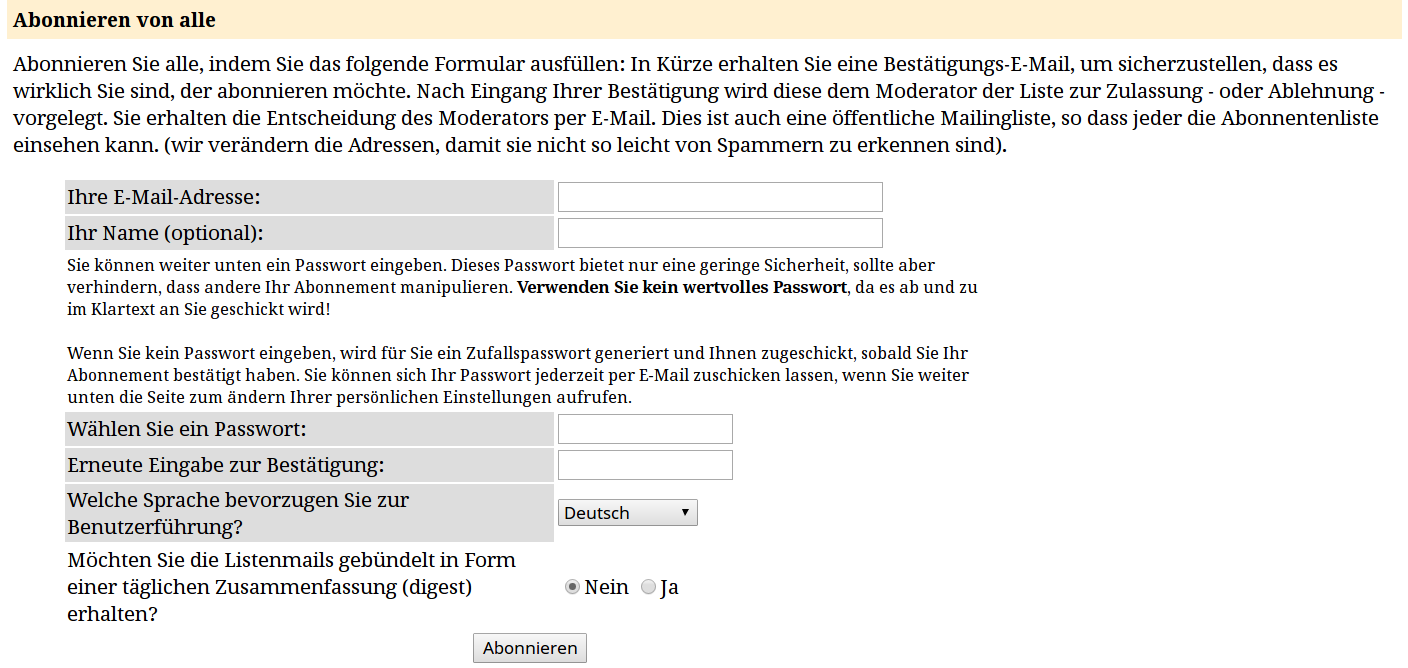
\includegraphics[width=\textwidth]{../images/lists_abbonieren.png}
   \end{figure}
	}
\subsecframe{Optionen} {
	\begin{itemize}
		\item Login f\"ur Mitglieder
		\item K\"undigung des Abos
		\item Passwort zusenden
	\end{itemize}
	\url{https://lists.stura.htw-dresden.de/options/}\textbf{$<$Name der Liste$>$}
	
	}
\frame{
	\frametitle{Login f\"ur Mitglieder}
		Welche E-Mailverteiler habe ich abboniert?
   \begin{figure}
	   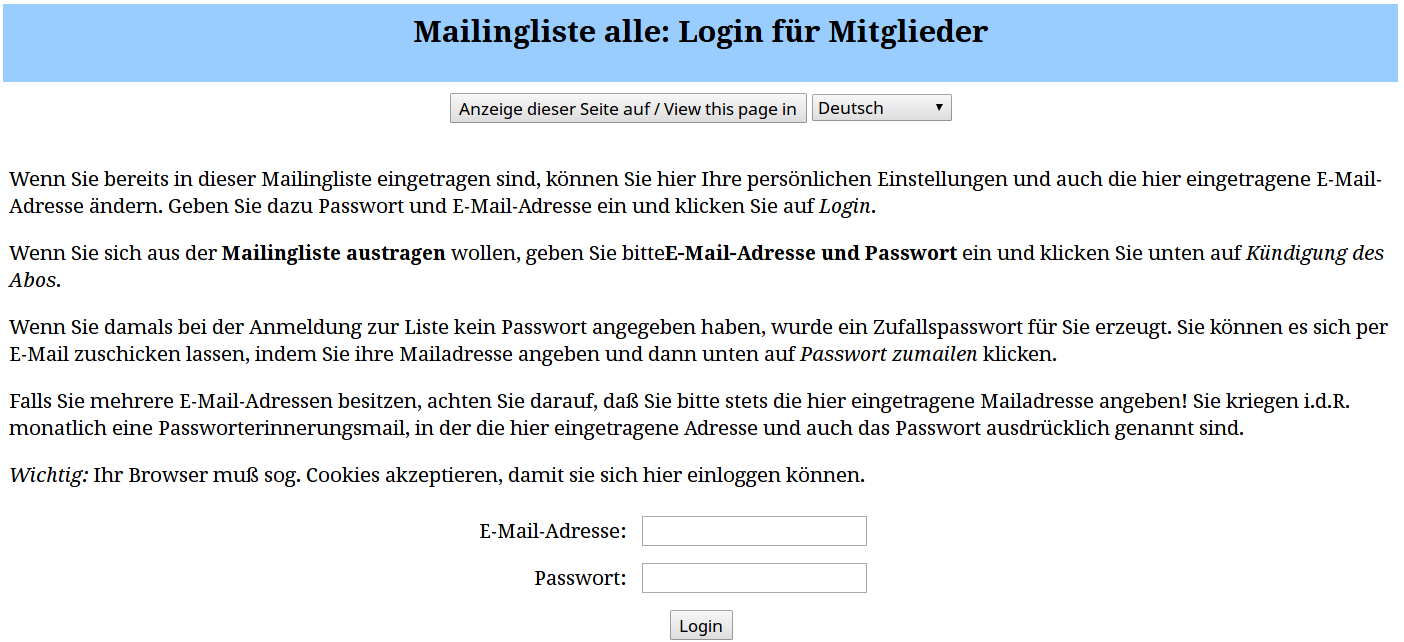
\includegraphics[width=\textwidth]{../images/lists_options.png}
   \end{figure}
   }

\frame{
	\frametitle{K\"undigung des Abos}
	M\"ochtest du die Liste abbestellen, dann trage unter \textbf{Login f\"ur Mitglieder} deine E-Mailadresse und dein Passwort ein und dr\"ucke dann auf \textit{K\"undigung des Abos}.
   \begin{figure}
	   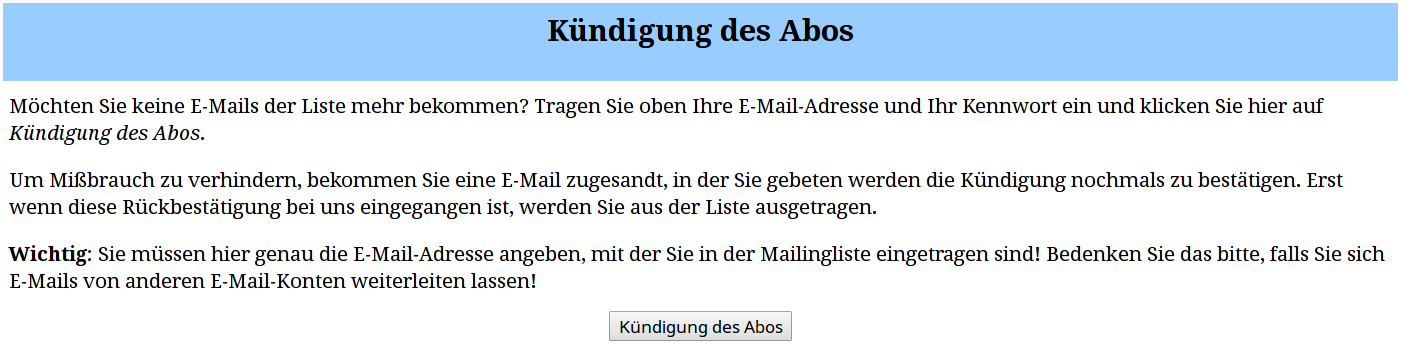
\includegraphics[width=\textwidth]{../images/lists_abbestellen.png}
   \end{figure}
}
\frame{
	\frametitle{Passwort zusenden}
	Hast du dein Passwort vergessen, dann trage unter \textbf{Login f\"ur Mitglieder} deine E-Mailadresse ein und dr\"ucke dann auf \textit{Passwort mailen}.
   \begin{figure}
	   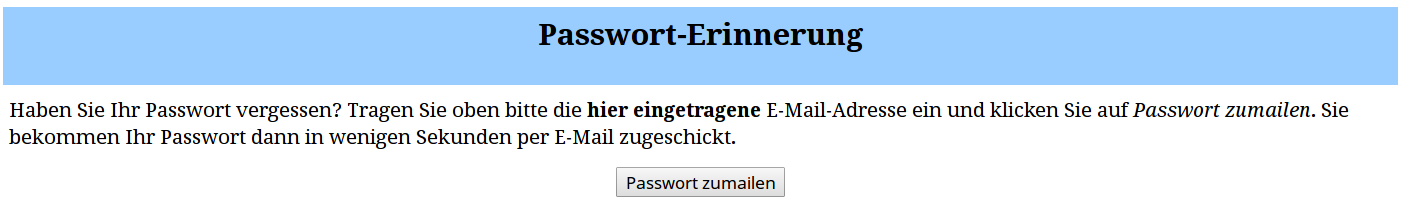
\includegraphics[width=\textwidth]{../images/lists_password_recover.png}
   \end{figure}
}
